The tasks of cleaving and polishing the fibers add a small dispersion in the individual scintillating fiber response to the instrinsic dispersion from fabrication. This generates an uncertainty, $\sigma_{sys-SF}$, which is the contribution of the fibers to the total uncertainty in the tritium activity measured by the TRITIUM detector. The setup shown in Figure \ref{fig:SetUpFiberCharacterization} was used to measure this uncertainty, in which has to be taken into account that the position of the connectors that lock the fiber in the experimental setup produces an additional systematic uncertainty, $\sigma_{sys-pos}$, in the measurement. Since both uncertainties are independent, the total systematic uncertainty is given by:

\begin{equation}
\sigma_{sys} = \sqrt{\sigma^2_{sys-SF} + \sigma^2_{sys-pos} }
\label{eq:TotalUncertaintyFiberCharacterization}
\end{equation}
The uncertainty due to the fiber position has to be quantified to extract $\sigma^2_{sys-SF}$ from the total systematic uncertainty. Two different experiments were designed, the first giving only the systematic uncertainty ($\sigma_{t} = \sigma_{sys}$), and the second to obtain the total uncertainty. Then, $\sigma^2_{sys-SF}$ is given by,

\begin{equation}
\sigma_{sys-SF} = \sqrt{\sigma^2_{sys} - \sigma^2_{sys-pos} }
\label{eq:TMUncertaintyFiberCharacterization}
\end{equation}
The test designed to measure $\sigma_{sys-pos}$ consisted in preparing one fiber of each type (uncladded, single clad and multiclad), all with $1~\mm$ diameter and $20~\cm$ length, using the conditioning process reported in section \ref{subsec:SurfaceConditioningProcess}. Each fiber was locked in the setup, and measurements of the PMT photocurrent with a fixed LED intensity, polarized at $1~\milli\ampere$ were made. These measurements were repeated ten times with a given fiber, removing and putting on the fiber each time. The mean, $\bar{x}$, and the standard deviation of the PMT photocurrent for each fiber type are shown in Table \ref{tab:PositionStandardDeviation} where the relative standard deviation, $\sigma^{rel}_{sys-pos}$, defined by equation \ref{eq:RelativeStandardDesviation}, is also included.

\begin{equation}
\sigma^{rel}_{sys} = \frac{\sigma_{sys-pos}}{\bar{x}}
\label{eq:RelativeStandardDesviation}
\end{equation}

\begin{table}[htbp]
\centering{}%
\begin{tabular}{lccc}
\toprule 
Fiber type & Mean ($\text{ph}$/ns) & $\sigma_{sys}$ ($\text{ph}$/ns) & $\sigma^{rel}_{sys}$ (\%) \tabularnewline
\midrule
\midrule 
Uncladded & $524.09 \pm 0.01$ & $17.65$ & $3.37$ \tabularnewline
Single Clad & $1071.70 \pm 0.01$ & $9.07$ & $0.85$ \tabularnewline
Multiclad & $949.93 \pm 0.03$ & $9.91$ & $1.04$ \tabularnewline
\bottomrule
\end{tabular}
\caption{Mean and standard deviation (due to the fiber position in the setup) of the number of photons per nanosecond that reach the PMT for $0.1~\milli\ampere$ LED intensity.}
\label{tab:PositionStandardDeviation}
\end{table}
%As it can be noticed, the clad reduces the position uncertainty, which means that it improves the uniformity of the fiber response. It was also found that 
As it can be noticed, the clad significantly improves the light collection efficiency of the fibers, showing larger signals for single clad fibers and multiclad fibers than for uncladded fibers. The reason could be that the interface between the core of the fiber and its clad is better controlled for single-clad and multi-clad fibers than for uncladded fibers, where the interface is provided by the environment (air or water in the case of TRITIUM). External conditions, as dirt, may produce noticeable interface fluctuations. It is also seen in the table that a second clad slightly reduces the collection efficiency. The reason could be that a second clad layer reduces the radius of the fiber core proportionally, keeping the external diameter at $1~\mm$. Concerning the statistical error of the measurement, it is three orders of magnitude smaller than the systematic uncertainties previously mentioned ($\sigma_{sys-pos}$ and $\sigma_{sys-SF}$) so it was negligible.

%In addition to the $\sigma_{pos}$ measurement, we have measured the number of photons collected by each type of fiber in the same situation, which is higher for single clad and even higher for multiclad. It means that the clad has an appreciable effect on the fiber collection efficiency and it could be a possible point to futur studies.

To determine the total uncertainty, ten different samples of each fiber type were prepared and each fiber was measured under the same conditions as above. This measurement was done for four different LED emission intensities ($0.05$, $0.1$, $0.15$ and $0.2~\milli\ampere$). The results for uncladded fibers are plotted in Figure \ref{fig:10samplesNC}, where it can be seen that, although each fiber shows a very linear trend with increasing LED emission intensity, a dispersion in the fiber response is clearly observed. Similar results were obtained for single clad and multiclad fibers, displayed in figures \ref{subfig:10samplesSC} and \ref{subfig:10samplesMC}, respectively.

\begin{figure}[h]
\centering
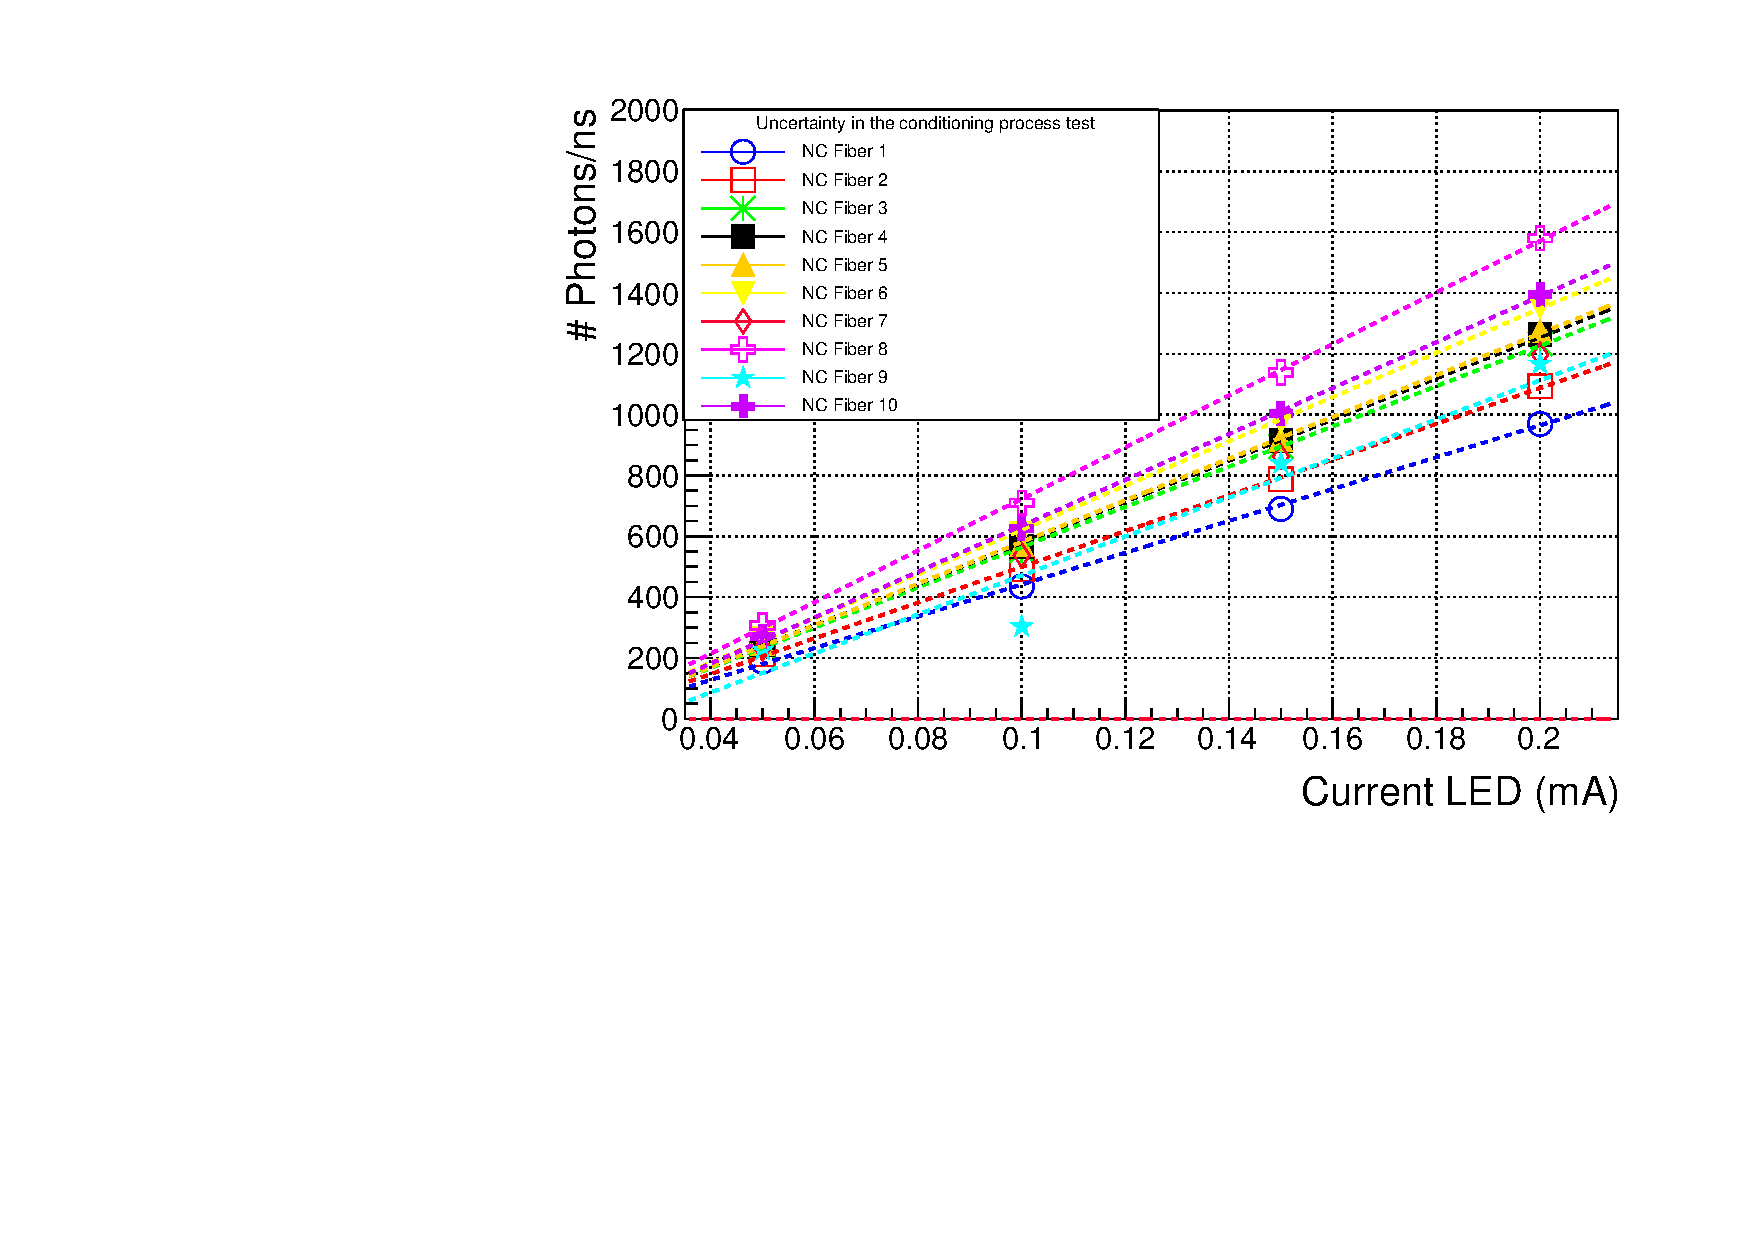
\includegraphics[scale=0.7]{4ResearchAndDevelopments/41Fibers/10_Different_samples_NoClad.pdf}
\caption{Number of photons/ns reaching the PMT for Uncladded fibers. Error bars are included but they are too small to be visible.\label{fig:10samplesNC}}
\end{figure}

\begin{figure}
\centering
    %\begin{subfigure}[b]{0.6\textwidth}
    %\centering
    %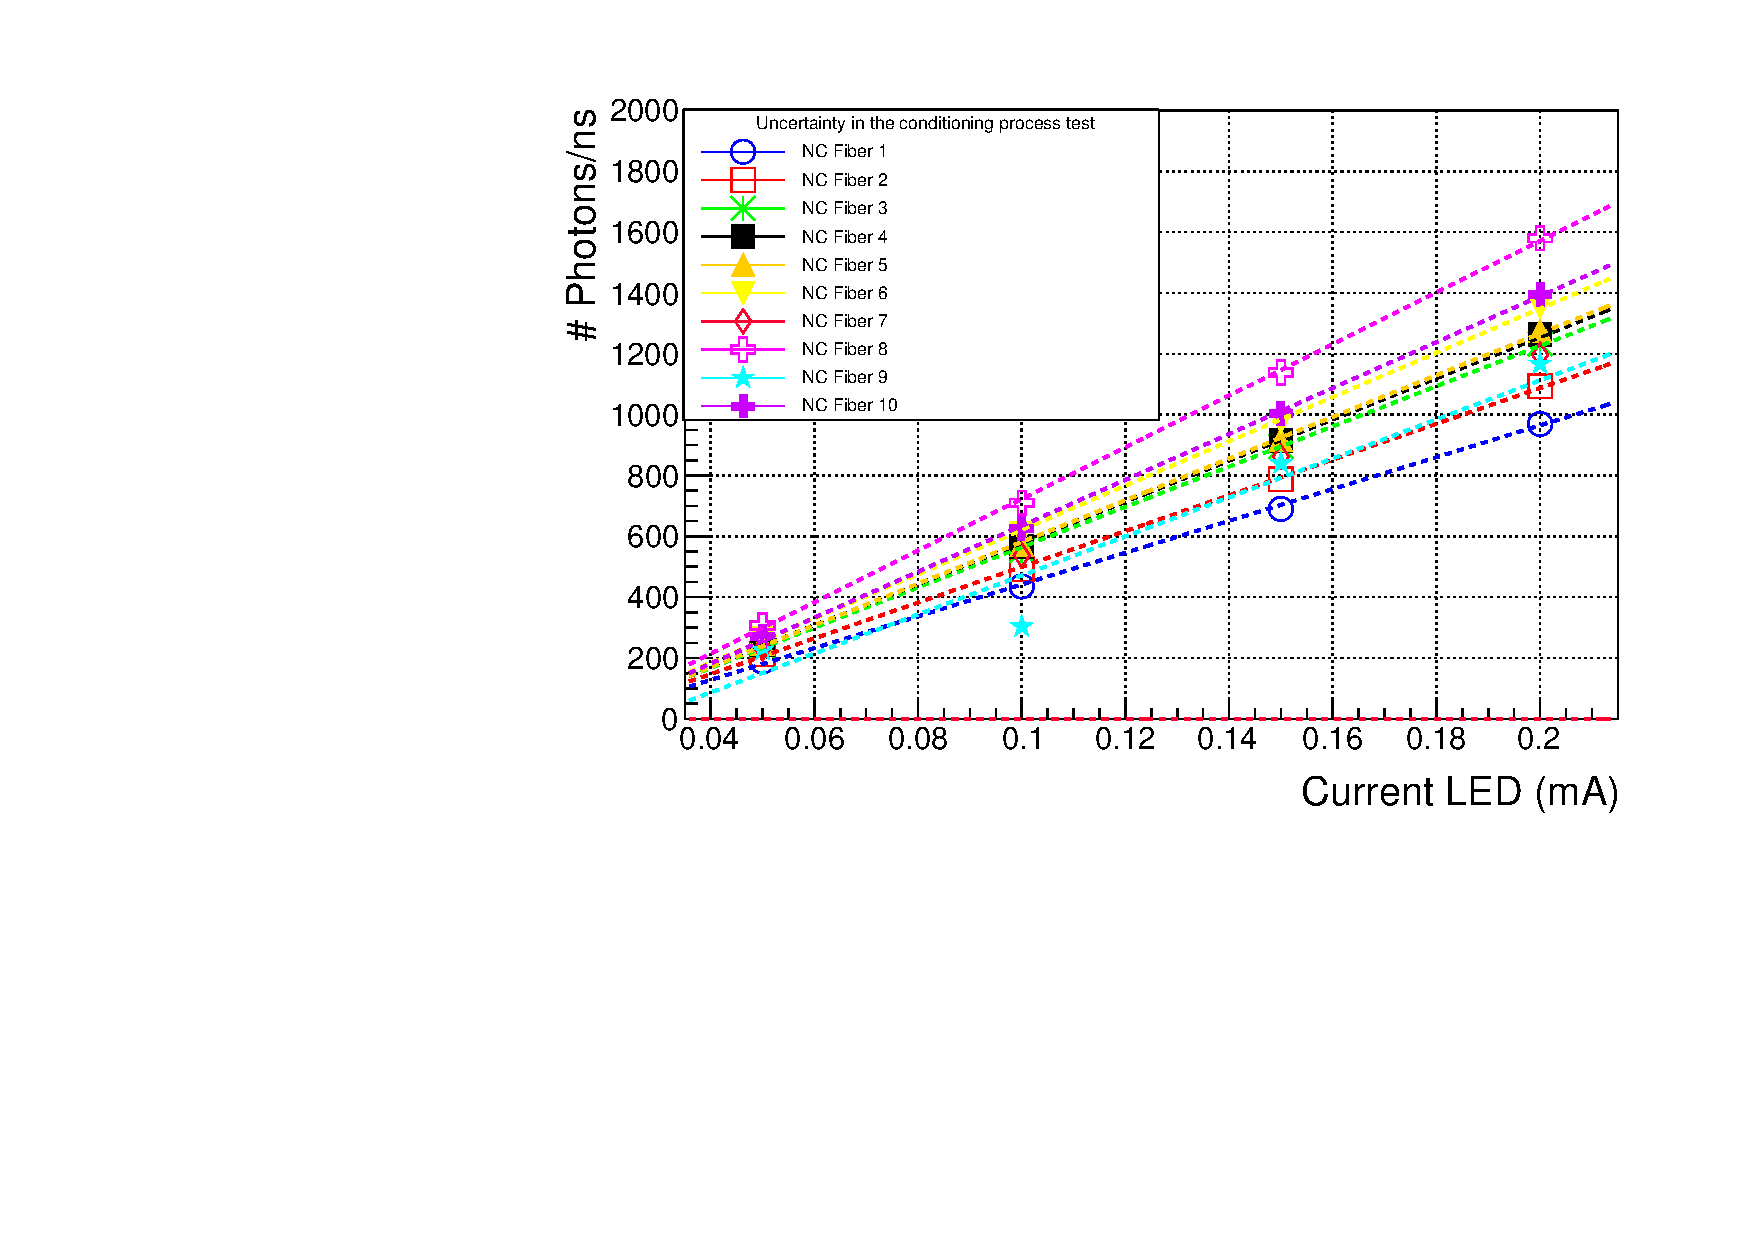
\includegraphics[width=\textwidth]{4ResearchAndDevelopments/41Fibers/10_Different_samples_NoClad.pdf}  
    %\caption{Number of photons/ns reaching the PMT for uncladded fibers.\label{subfig:10samplesNC}}
    %\end{subfigure}
    %\hfill
    \begin{subfigure}[b]{1\textwidth}
    \centering
    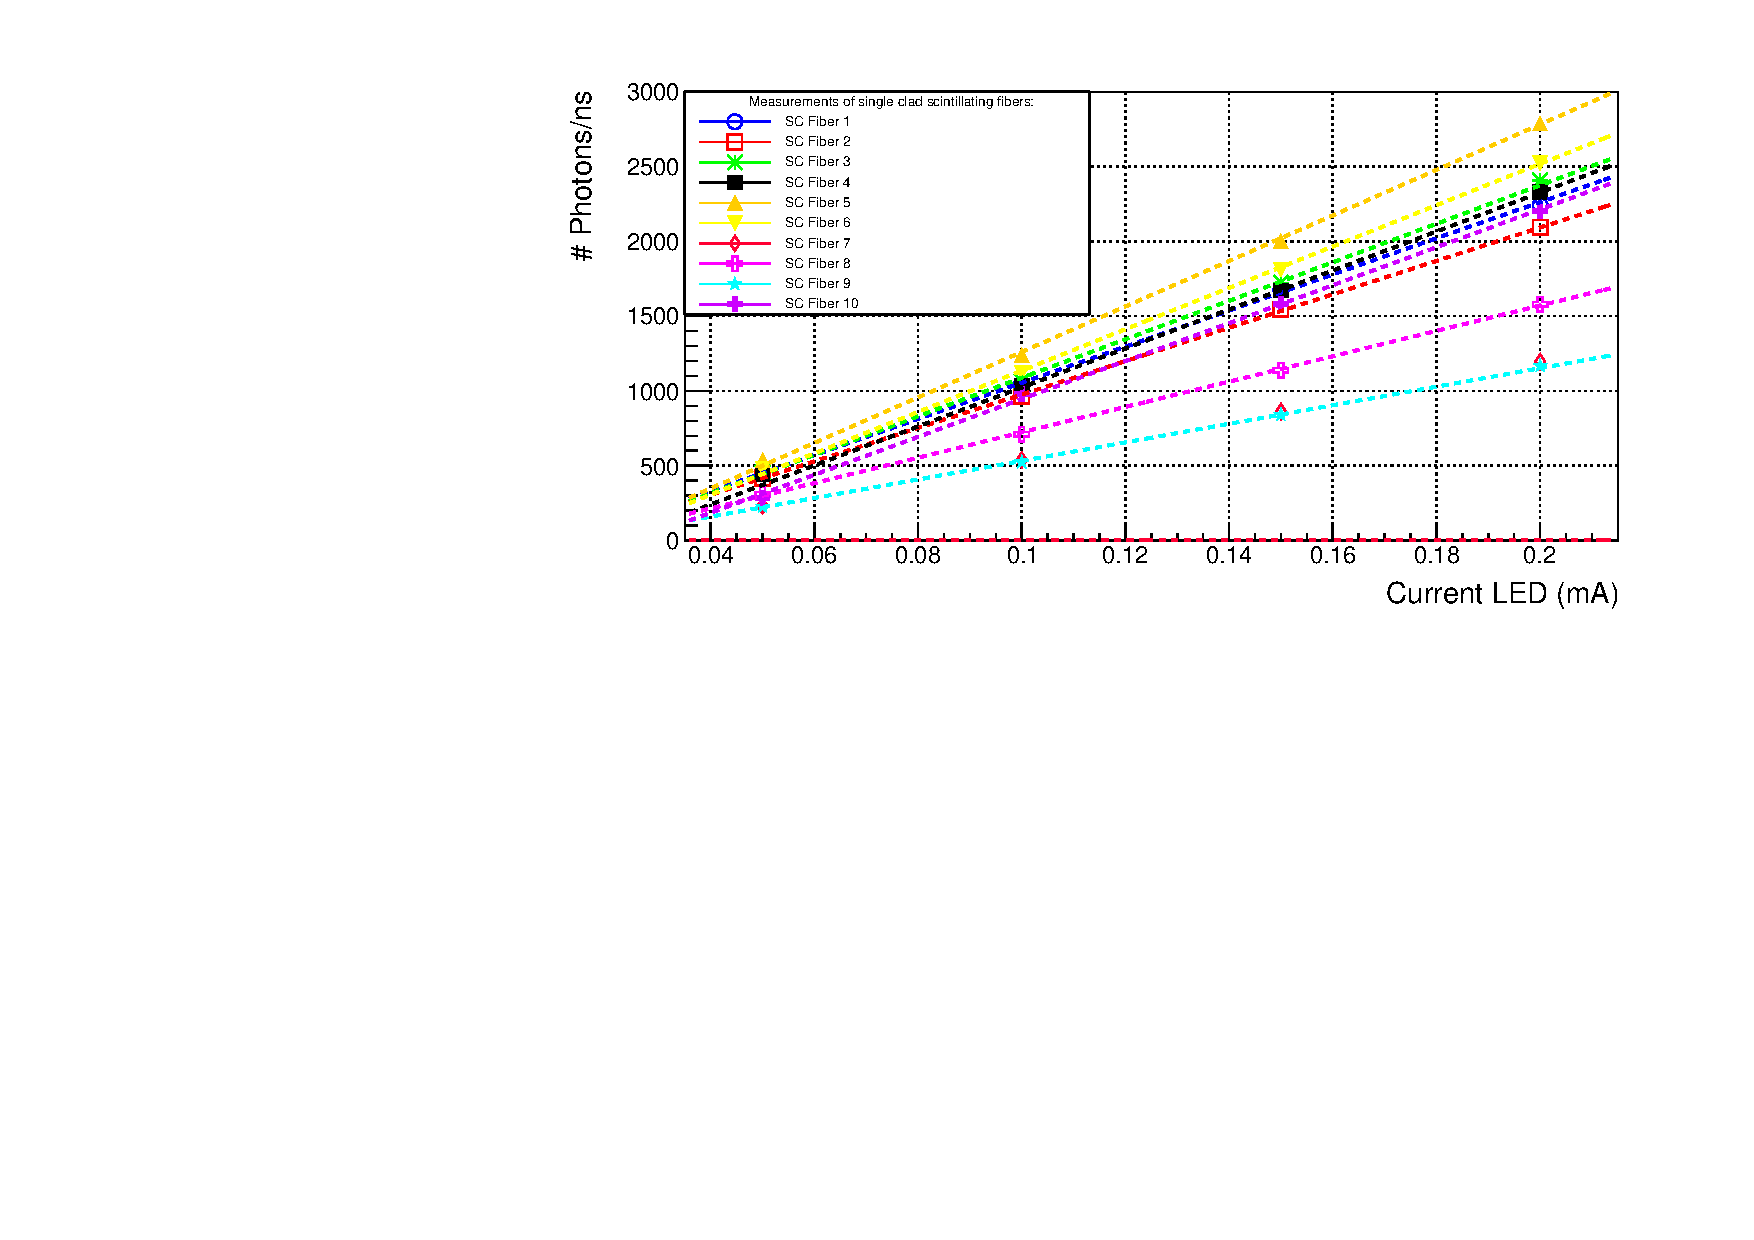
\includegraphics[width=\textwidth]{4ResearchAndDevelopments/41Fibers/10_Different_samples_SingleClad.pdf}  
    \caption{\label{subfig:10samplesSC}}
    \end{subfigure}
    \hfill
    \begin{subfigure}[b]{1\textwidth}
    \centering
    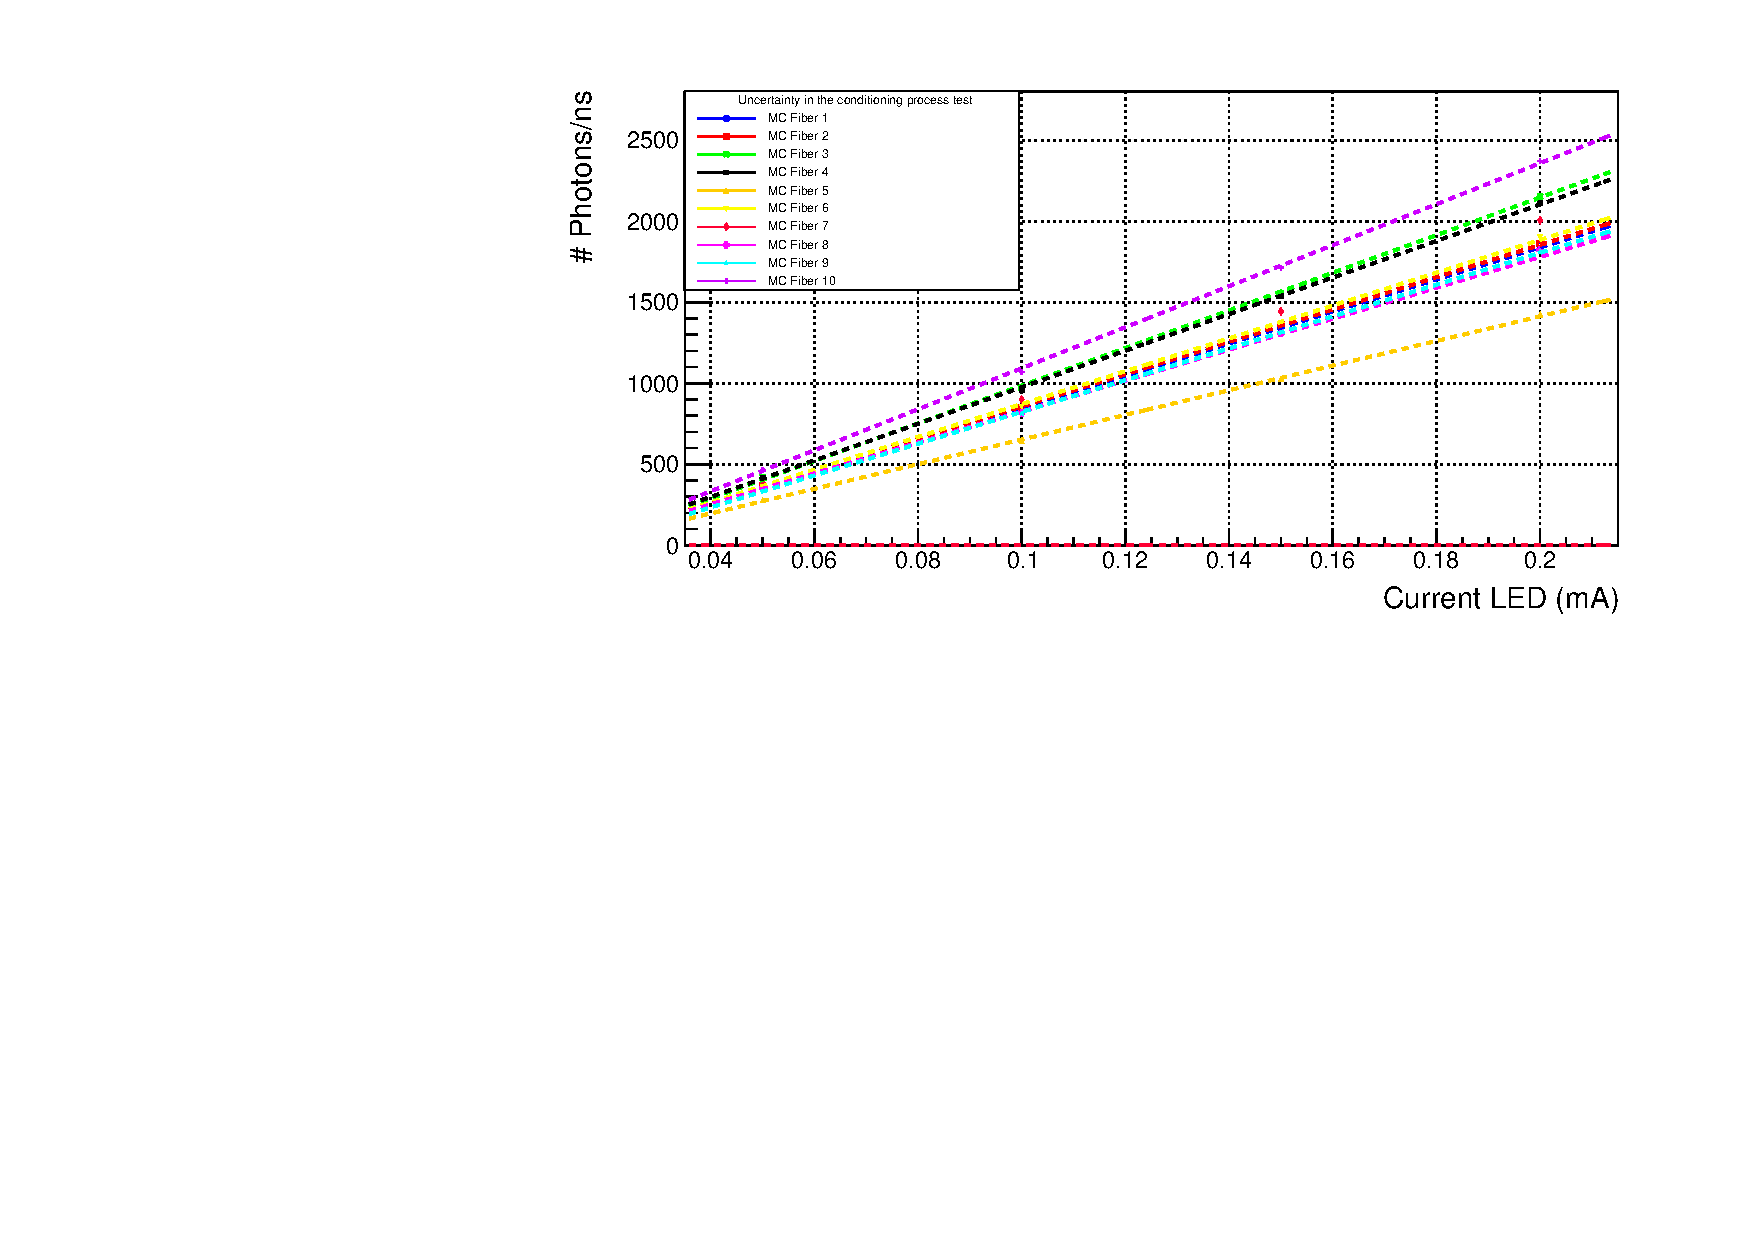
\includegraphics[width=\textwidth]{4ResearchAndDevelopments/41Fibers/10_Different_samples_MultiClad.pdf}  
    \caption{\label{subfig:10samplesMC}}
    \end{subfigure}
 \caption{Number of photons/ns reaching the PMT for ten samples. a) Single clad fibers, b) Multi-clad fibers. Error bars are included but they are too small to be visible.}
 \label{fig:10samplesThreeTypes}
\end{figure}
The average number of collected photons versus LED intensity and the relative standard deviation for each type of fiber are given in Tables \ref{tab:10DifferentSamples} and \ref{tab:RelativeStandardDeviation3FiberTypes} respectively, and are plotted in Figure \ref{fig:AveregeThreeFiberTypes}, where they can be compared. 

\begin{table}[h]
\centering{}%
\begin{tabular}{lccc}
\toprule 
Led Int. (mA) & Uncladded ($\text{ph}/\nano\second$) & Single Clad ($\text{ph}/\nano\second$) & MultiClad ($\text{ph}/\nano\second$) \tabularnewline
\midrule
\midrule 
$0.05$ & $245 \pm 11$ & $384 \pm 33$ & $377 \pm 15$ \tabularnewline
$0.1$ & $572 \pm 26$ & $923 \pm 74$ & $871 \pm 35$ \tabularnewline
$0.15$ & $915 \pm 39$ & $1485 \pm 120$ & $1397 \pm 55$ \tabularnewline
$0.2$ & $1267 \pm 55$ & $2054 \pm 166$ & $1933 \pm 76$ \tabularnewline
\bottomrule
\end{tabular}
\caption{Number of collected photons per nanosecond versus LED intensity for the different type of fibers. The errors shown here are the standard deviation of the ten measured samples.}
\label{tab:10DifferentSamples}
\end{table}

\begin{table}[h]
\centering{}%
\begin{tabular}{lccc}
\toprule 
Led Int. (mA) & Uncladded (\%) & Single Clad (\%) & MultiClad (\%) \tabularnewline
\midrule
\midrule 
$0.05$ & $4.38$ & $8.66$ & $3.97$ \tabularnewline
$0.1$ & $4.59$ & $8.02$ & $3.97$ \tabularnewline
$0.15$ & $4.34$ & $8.07$ & $3.95$ \tabularnewline
$0.2$ & $4.36$ & $8.10$ & $3.93$ \tabularnewline
\midrule 
Mean & $4.42$ & $8.21$ & $3.96$ \tabularnewline
\bottomrule
\end{tabular}
\caption{Relative standard deviation, $\sigma^{rel}_t(\%)$, versus LED intensity for the different fiber types.}
\label{tab:RelativeStandardDeviation3FiberTypes}
\end{table}

\begin{figure}[h]
\centering
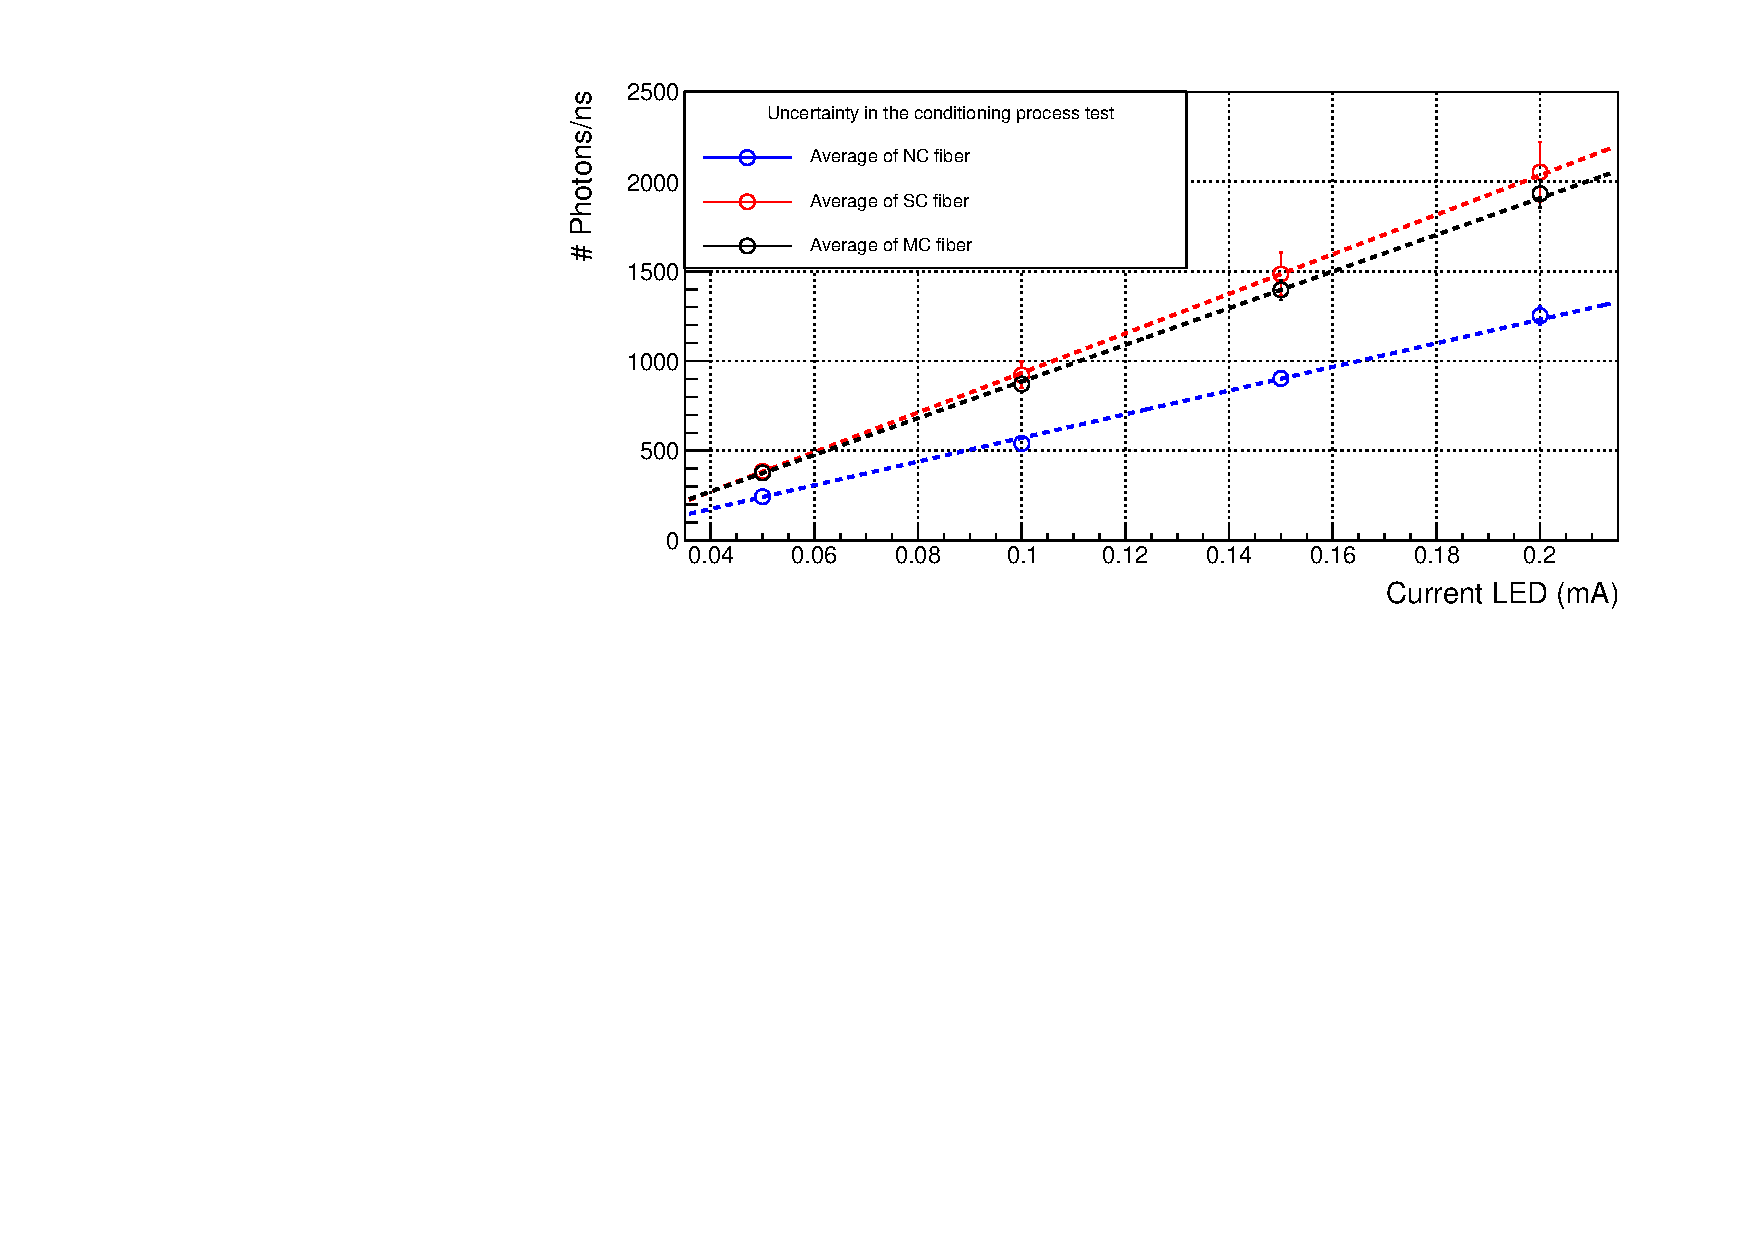
\includegraphics[scale=0.6]{4ResearchAndDevelopments/41Fibers/10_Different_Samples_Average_3_Fiber_Types.pdf}
\caption{Average number of photons per ns versus LED current for 10 samples of each fiber type (uncladded, single clad and multi-clad fibers). Error bars are included but they are too small to be visible.\label{fig:AveregeThreeFiberTypes}}
\end{figure}

As it can be noticed in Figures \ref{fig:10samplesNC} and \ref{fig:10samplesThreeTypes}, the fiber response is quite linear and single clad and multiclad fibers have stronger signals than uncladded fibers, which indicates, as already observed in Table \ref{tab:PositionStandardDeviation}, that the clad has a significant effect on the fiber collection efficiency. It can also be observed in Table \ref{tab:RelativeStandardDeviation3FiberTypes} that the relative standard deviation, $\sigma^{rel}_{sys}$, does not vary with the LED intensity. The highest uncertainty was found for the single-clad fibers, despite of their higher light collection. This is most probably due to the cleaving process during which cracks in the clad my appears as it cas be observed in Figure \ref{fig:CleavingFiberEnd}. As can be observed in Table \ref{tab:RelativeStandardDeviation3FiberTypes}, this damage seems to be reduced when a second clad is used, which enhances the mechanical resistance of the fiber.

%The relative standard deviation are also presented in these tables, where we it can be seen that the dispersion of each fiber type for different LED intensities is practically negligible, which again verifies the correct behavior of the system. 

%There is only one point (uncladded fiber with $0.1~\milli\ampere $) that is higher than we expect. We can see in Table \ref{tab:10DifferentSamplesNoClad} that the reason for this is that its standard deviation is too high (as high as the measurement for uncladded fibers with $0.15~\milli\ampere$). The reason was found in the sample 9, whose measurement was very different from the average, incresing the standard deviation, probably due to a problem in the measurement process. We discard this sample because this result is not representative.

An average of the three relative standard deviation quoted in this section, $\sigma^{rel}_{sys}$, $\sigma^{rel}_{sys-pos}$ and $\sigma^{rel}_{sys-SF}$,  are given in Table \ref{tab:RelativeStandardDeviations}. As it can be noticed, the smallest relative standard deviation was found for uncladded fibers, which means that the damage from this process occurs mainly in the fiber clad, as illustrated in Figure \ref{fig:ResultofPolishingProcess} where it can seen the clad break due to the cleaving process. It was checked under microscope that this damage only occurs at the end of the fiber. Also, the largest relative standard deviation is obtained for single clad fibers, which indicates that the second clad increases the resistance of the fiber to the conditioning process.

\begin{table}[htbp]
\centering{}%
\begin{tabular}{lccc}
\toprule 
Fiber type & $\sigma_{sys}$ (\%) & $\sigma_{sys-pos}$ (\%) & $\sigma_{sys-SF}$ (\%) \tabularnewline
\midrule
\midrule 
Uncladded & $4.42$ & $3.37$ & $2.86$ \tabularnewline
Single Clad & $8.21$ & $2.17$ & $7.92$ \tabularnewline
Multiclad & $3.96$ & $1.04$ & $3.82$ \tabularnewline
\bottomrule
\end{tabular}
\caption{Relative standard deviations ($\sigma_{sys}$, $\sigma_{sys-pos}$ and $\sigma_{sys-SF}$) measured in this test.}
\label{tab:RelativeStandardDeviations}
\end{table}

In summary, the relative statistical deviation due to the fiber conditioning process was quantified for the different fiber types. It was found that the use of a fiber cladding improves the efficiency of photon collection but at the cost of worsening the standard deviation. Larger uncertainties (a factor two) in the light collection was observed in single clad fibers compared to multiclad and uncladded ones. This may be due to the damage in the clad produced during the cleaving process of these fibers. Therefore, it was chosen not to use a clad for the fibers used in the TRITIUM detector.

Finally, the absolute photon collection efficiency per meter, $CE_{100}$, for each type of fiber was measured. To measure it, ten different samples of $10~\cm$ length were prepared for each fiber type and similar measurements of the photons collected were performed, which are summarized in Table \ref{tab:10DifferentSamplesAlltypes}.

\begin{table}[htbp]
\centering{}%
\begin{tabular}{lccc}
\toprule 
Led Int. (mA) & Uncladded ($\gamma$/ns) & Single-clad ($\gamma$/ns) & Multi-clad ($\gamma$/ns) \tabularnewline
\midrule
\midrule 
$0.05$ & $318 \pm 61$ & $550 \pm 71$ & $480 \pm 84$ \tabularnewline
$0.1$ & $736 \pm 143$ & $1270 \pm 164$ & $1111 \pm 193$ \tabularnewline
$0.15$ & $1184 \pm 232$ & $1984 \pm 231$ & $1777\pm 307$ \tabularnewline
$0.2$ & $1645 \pm 324$ & $2507 \pm 208$ & $2338 \pm 350$ \tabularnewline
\bottomrule
\end{tabular}
\caption{Number of the collected photons versus LED intensity for 10 different fibers of $10~\cm$ length.}
\label{tab:10DifferentSamplesAlltypes}
\end{table}
The collection efficiency of $10~\cm$ fiber length, $CE_{10}$, was calculated by comparing these photons collected to those measured for a fiber length of $20~\cm$. It is quite similar to the expected value considering an exponential attenuation of the signal in length as follow \cite{}.
%The collection efficiency  to $CE_{100}$ was calculated from $CE_{10}$ by assuming an exponential attenuation of the signal in length as follow \cite{}.

\begin{equation}
N_{ph}/\nano\second(x) = N_{ph}/\nano\second(x_0) \times e^{-(x-x_0)/L}
\label{eq:ExponentialAttenuation}
\end{equation}

\begin{equation}
CE_{10}=\frac{N_{ph}/\nano\second(20~\cm)}{N_{ph}/\nano\second(10~\cm)}=e^{-10/L}=96\%
\label{eq:CollectionEfficiency}
\end{equation}
where L is the absortion length provided by the manufacturer, $L=260~\cm$. A lower collection efficiency has been obtained compared to the expected value for each type of scintillating fiber. This is likely due to blemishes and dirt on the fiber surface and a less than perfect interface between the fiber and the PMT used.

\begin{table}[htbp]
\centering{}%
\begin{tabular}{lcc}
\toprule 
Fiber type & $CE_{10}$ (\%) \tabularnewline
\midrule
\midrule 
UnCladded & $76 \pm 8$ \tabularnewline
Single Clad & $78 \pm 6$ \tabularnewline
Multiclad & $83 \pm 7$ \tabularnewline
\bottomrule
\end{tabular}
\caption{Collection efficiencies $CE_{10}$ and $CE_{100}$.}
\label{tab:CollectionEfficiencyOfFibers}
\end{table}


%The collection efficiency, $CE_{100}$, given by the manufacturer Saint-Gobain is in the range $3.44\%-7\%$ \cite{DataSheetBCF12Fiber}. Our measurements, given in Table \ref{tab:CollectionEfficiencyOfFibers}, are close but slightly higher than the manufacturer values which could be attributed to our use of collimated photons.

%As collimated photons were used in this study, the fact that our results are in the best side is justified. As it can be seen in Table \ref{tab:CollectionEfficiencyOfFibers}, our measured values are very close to those provided by the manufacturer. %The difference between this value for the three types of fiber studied is not as large as it was expected. A possible reason is that the difference in fiber length is only $10~\cm$ and it may not be enough to see this effect. It could be interesting to repeat these tests with a larger difference in fiber length.